\chapter{Diagramas das Microarquiteturas}\label{anexo_diagramas}

\begin{figure}[H]
\centering
    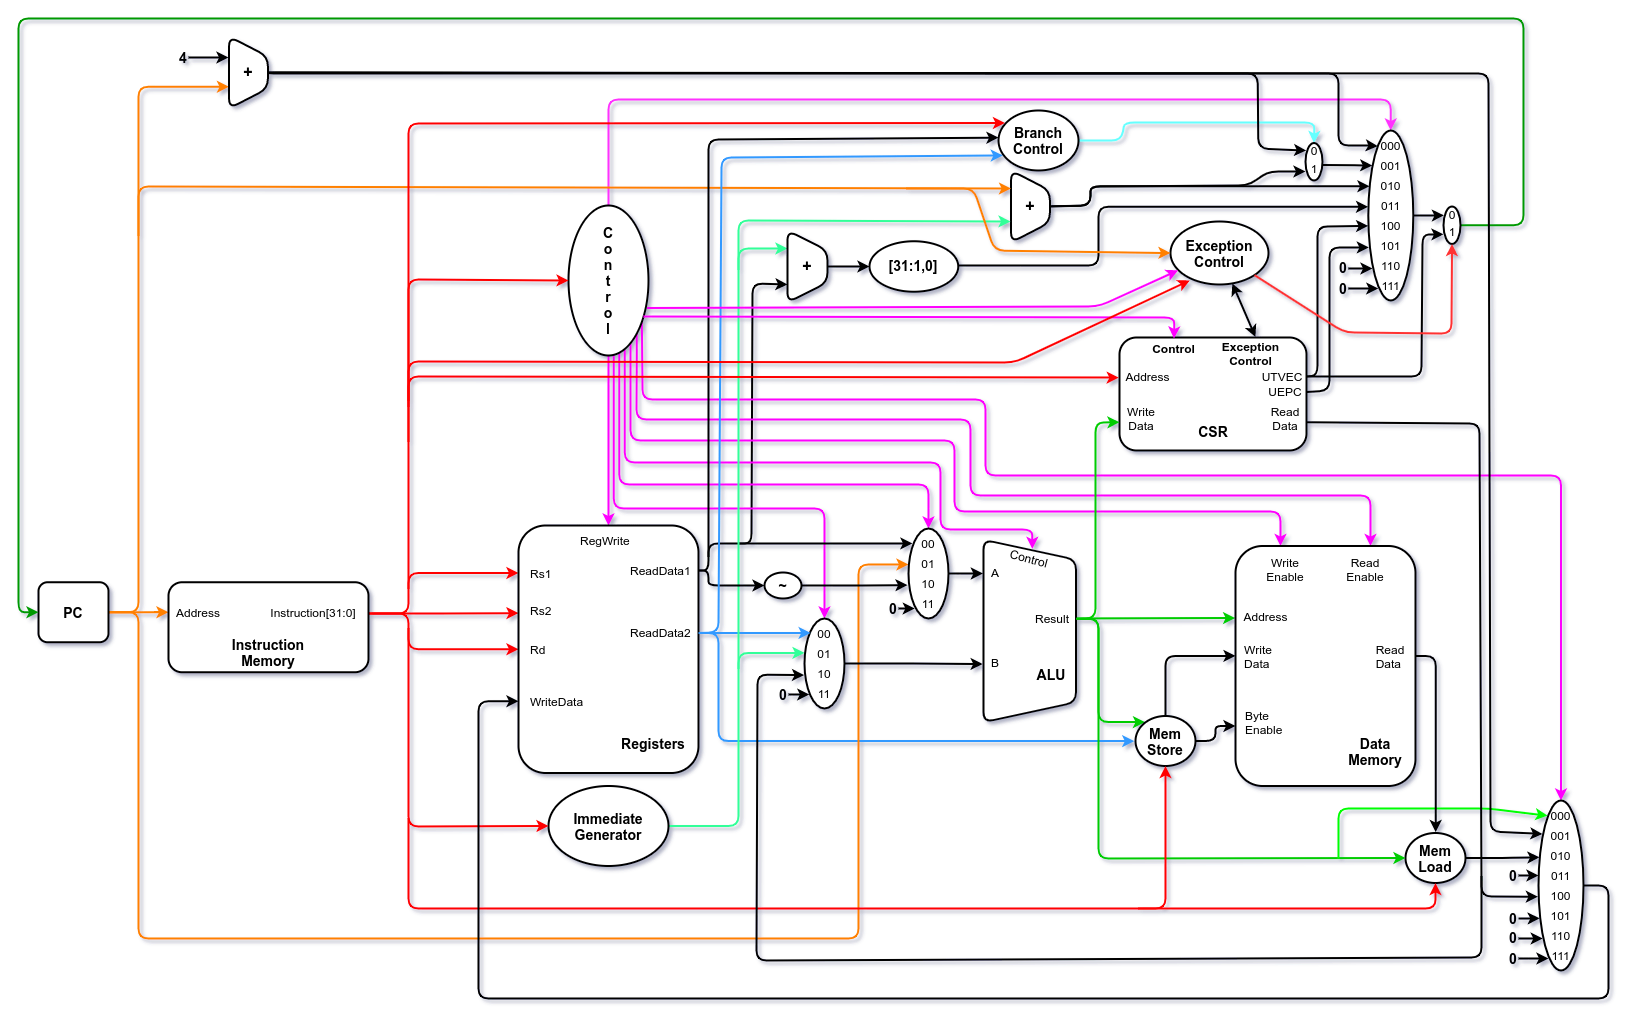
\includegraphics[angle=90,width=1\textwidth,height=.85\textheight,keepaspectratio]{../images/uarch_diagrams/singlecycle-RV32I-RV32IM.png}
    \caption{Diagrama do uniciclo \textit{RV32I e RV32IM}}
\end{figure}

\begin{figure}[H]
\centering
    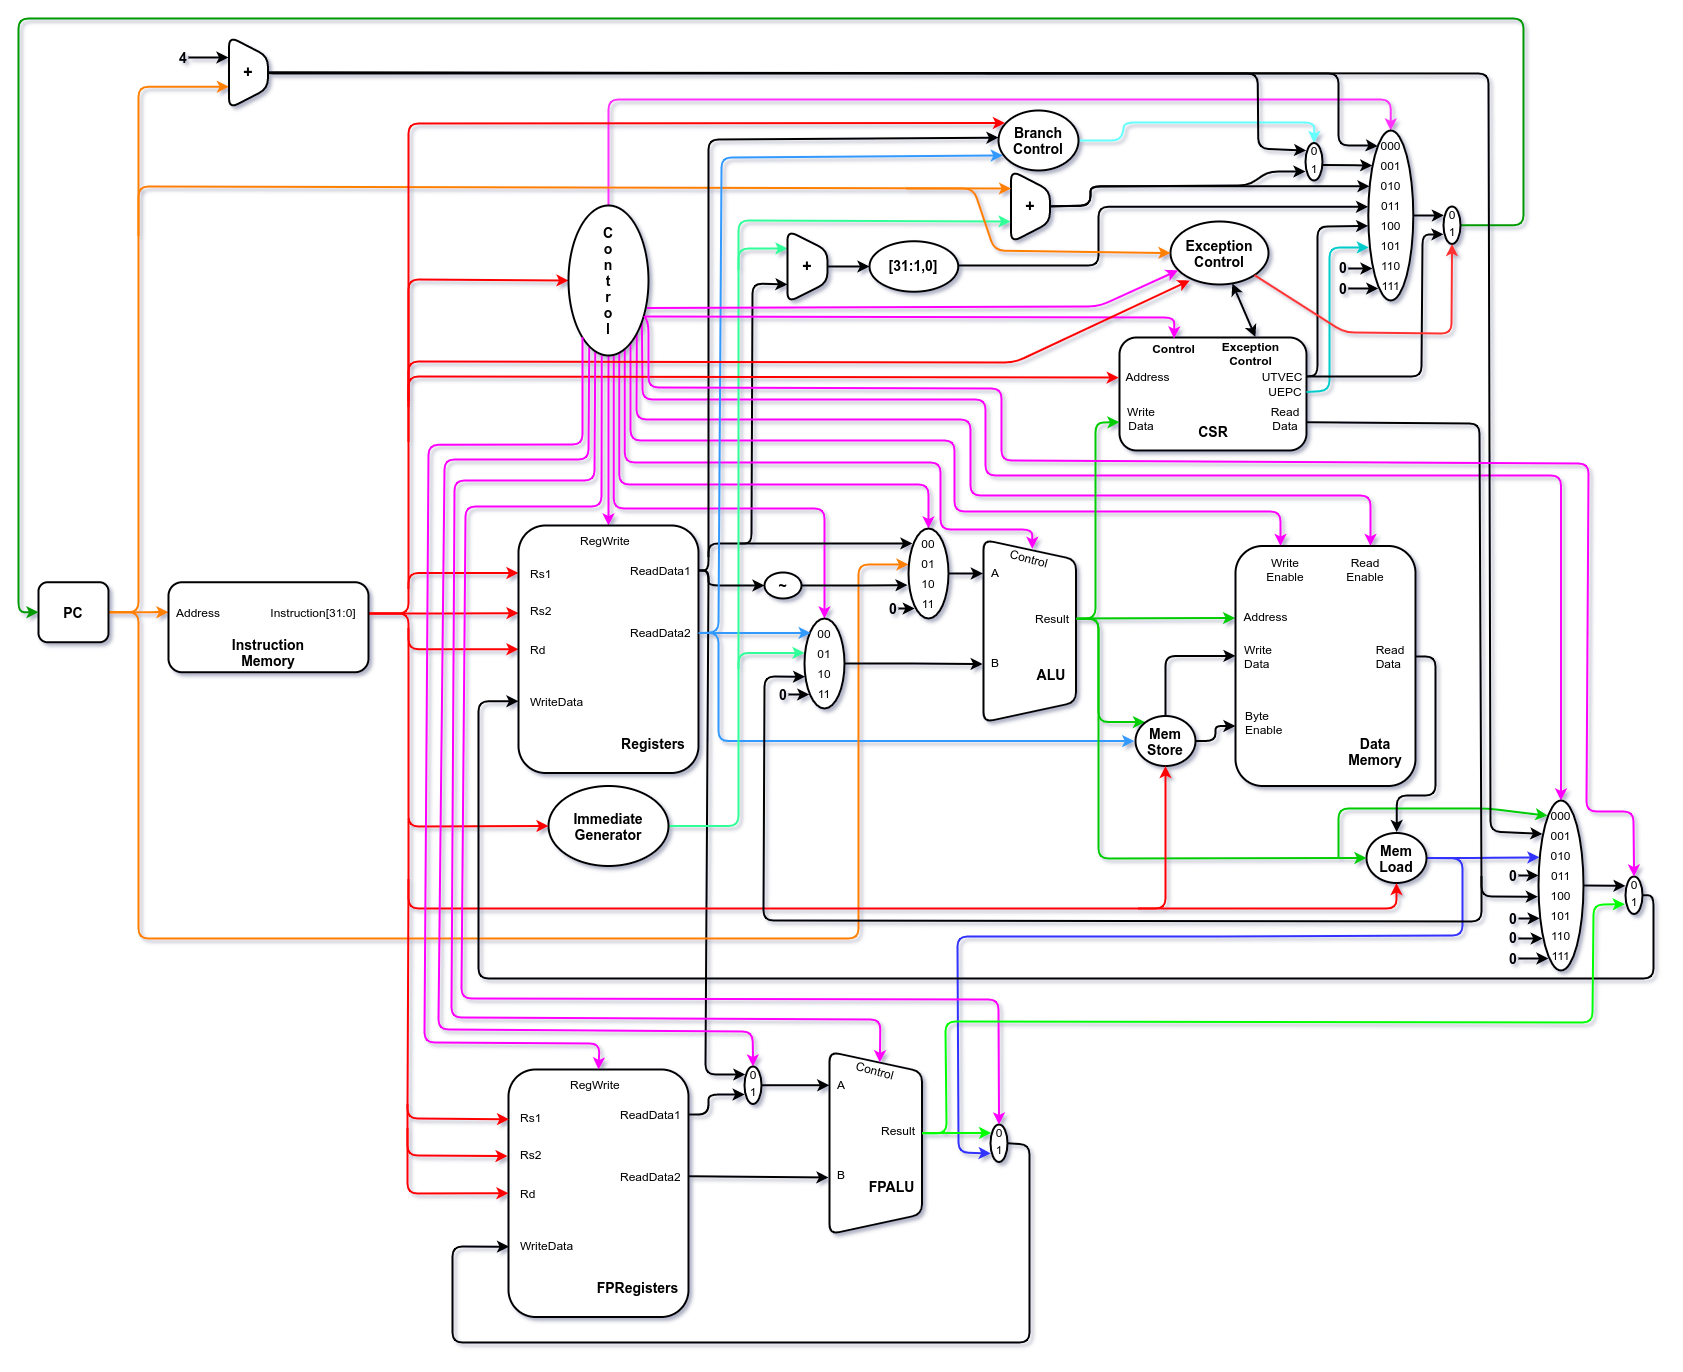
\includegraphics[angle=90,width=1\textwidth,height=1\textheight,keepaspectratio]{../images/uarch_diagrams/singlecycle-RV32IMF.png}
    \caption{Diagrama do uniciclo \textit{RV32IMF}}
\end{figure}

\begin{figure}[H]
\centering
    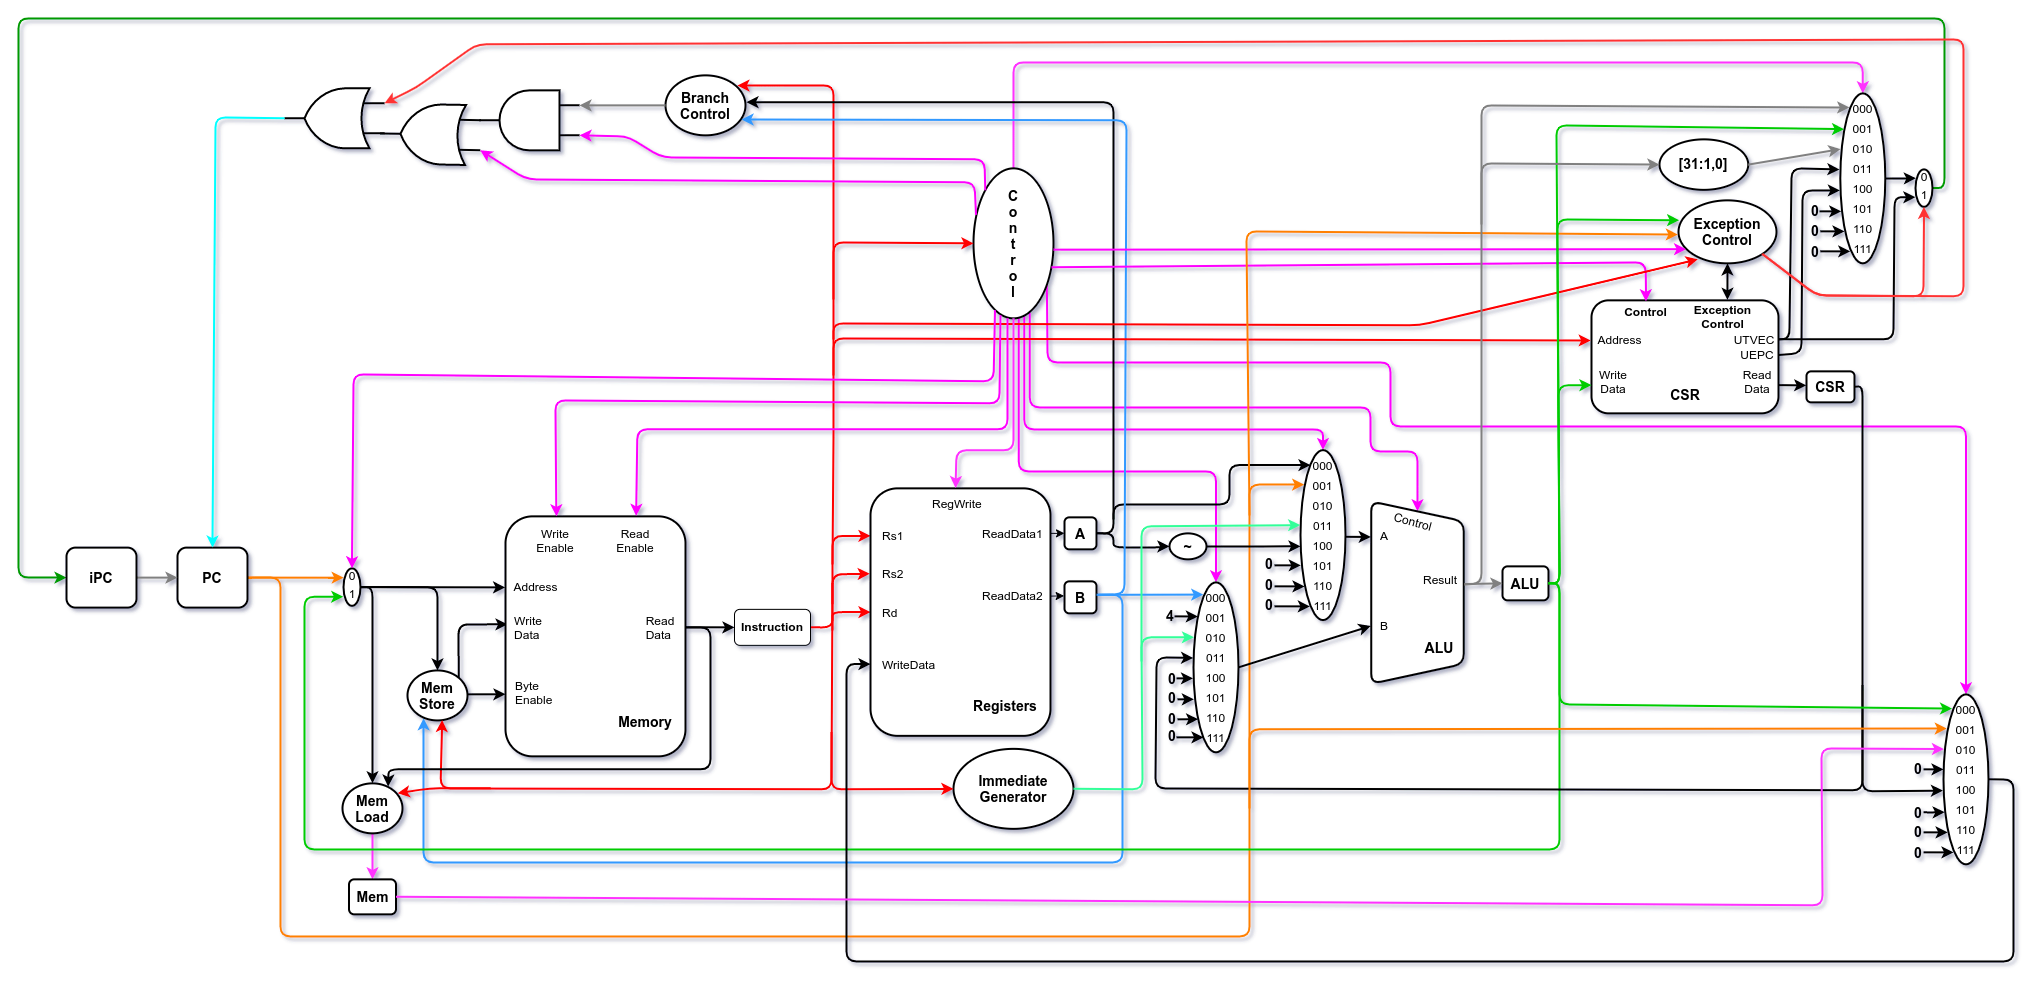
\includegraphics[angle=90,width=1\textwidth,height=1\textheight,keepaspectratio]{../images/uarch_diagrams/multicycle-RV32I-RV32IM.png}
    \caption{Diagrama do multiciclo \textit{RV32I e RV32IM}}
\end{figure}

\begin{figure}[H]
\centering
    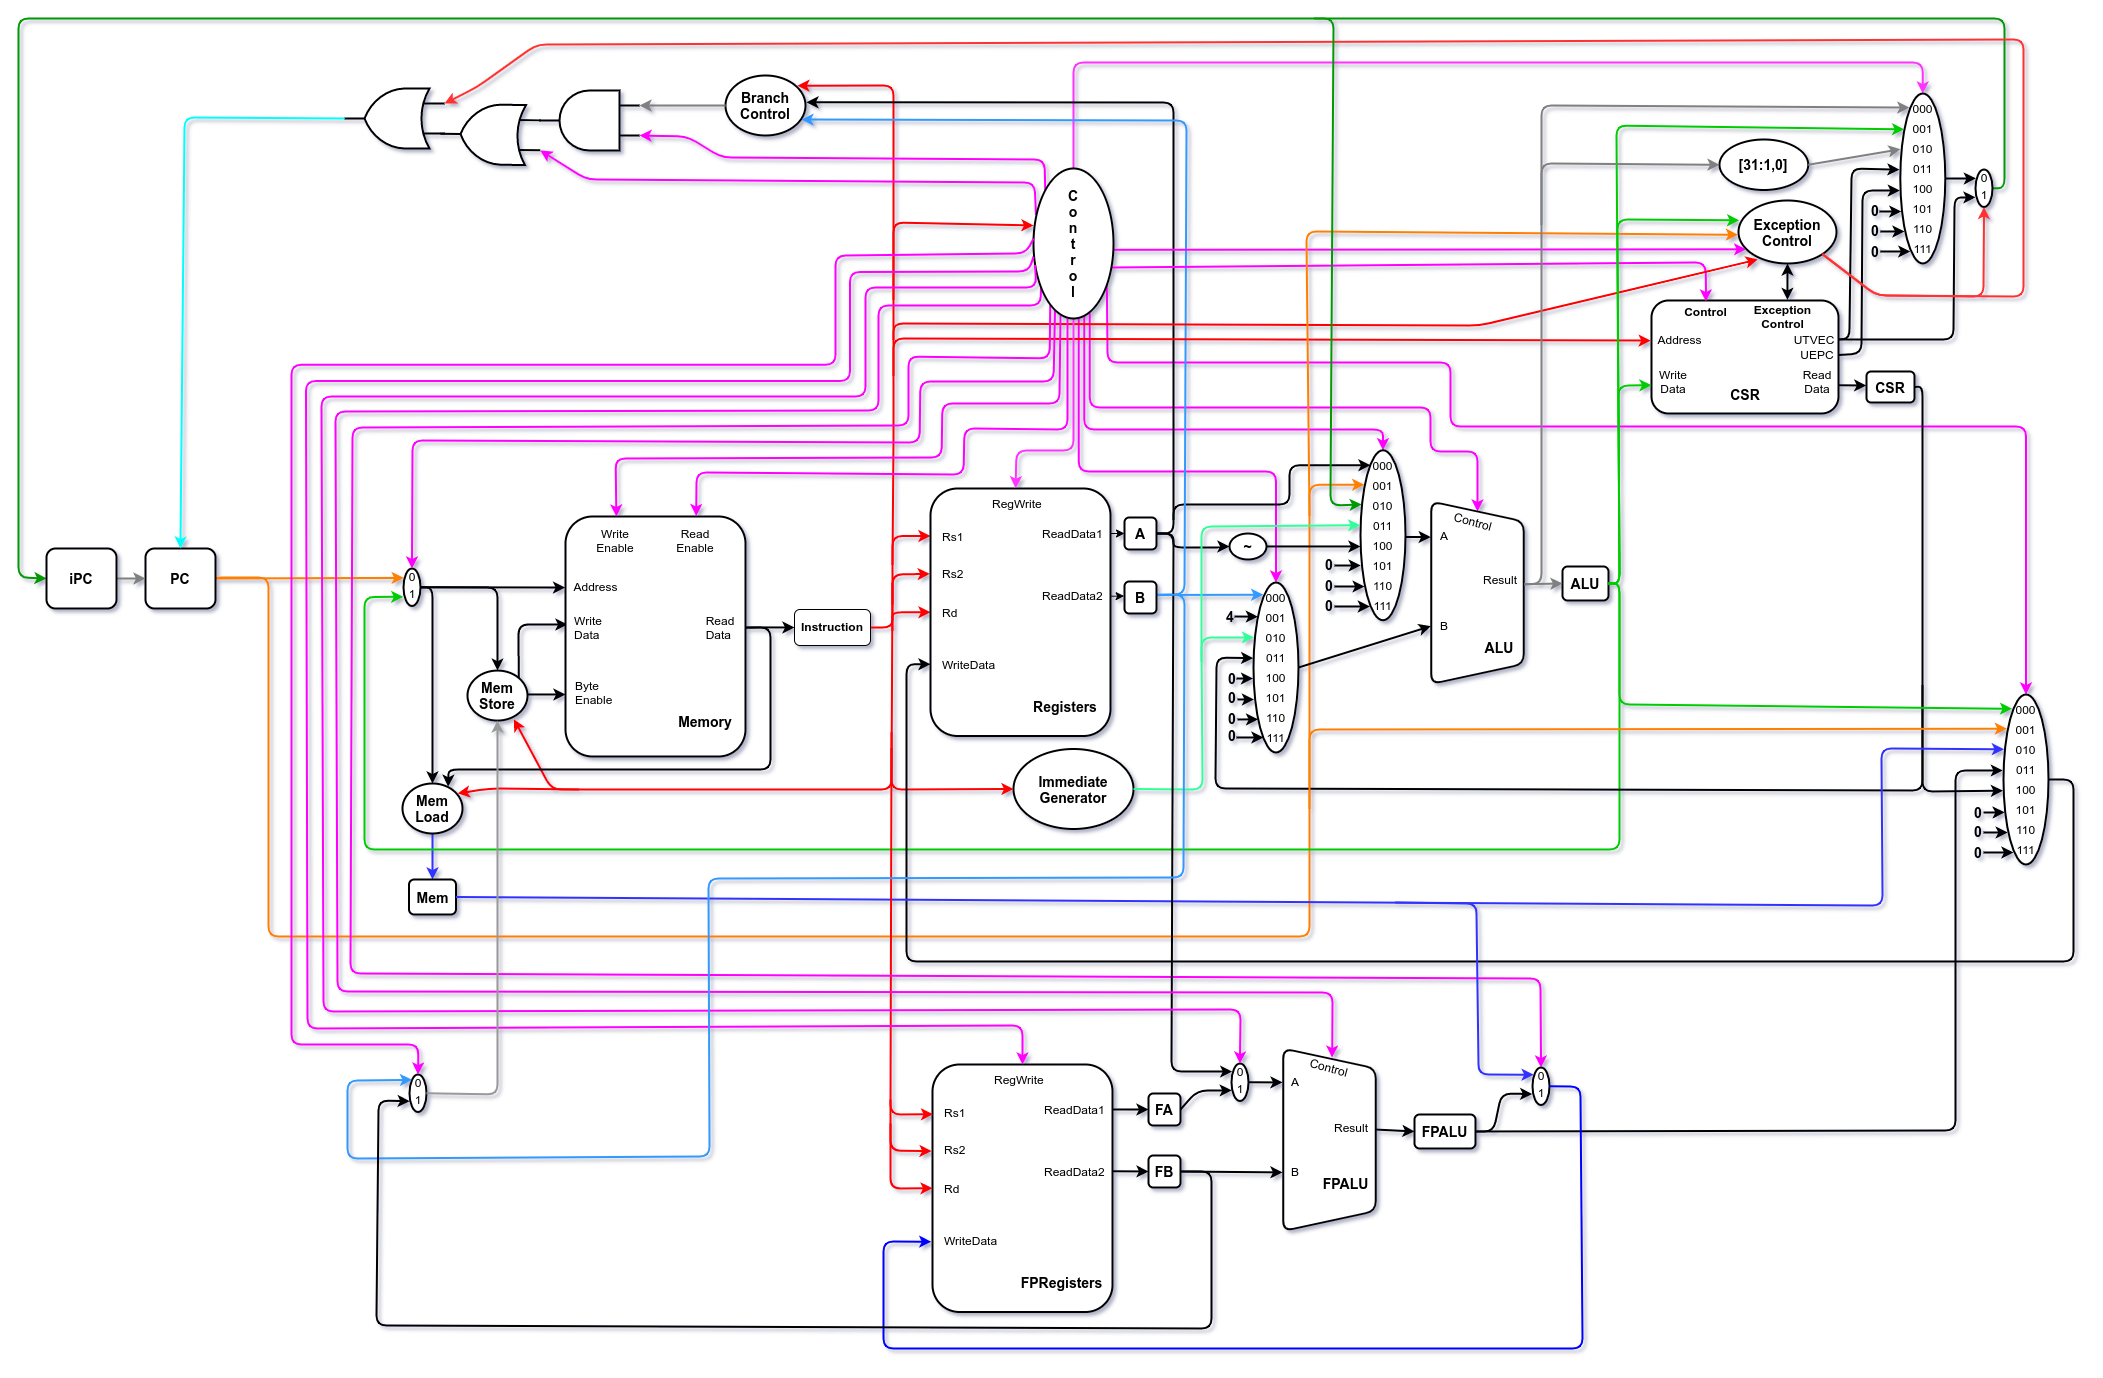
\includegraphics[angle=90,width=1\textwidth,height=1\textheight,keepaspectratio]{../images/uarch_diagrams/multicycle-RV32IMF.png}
    \caption{Diagrama do multiciclo \textit{RV32IMF}}
\end{figure}

\begin{figure}[H]
\centering
    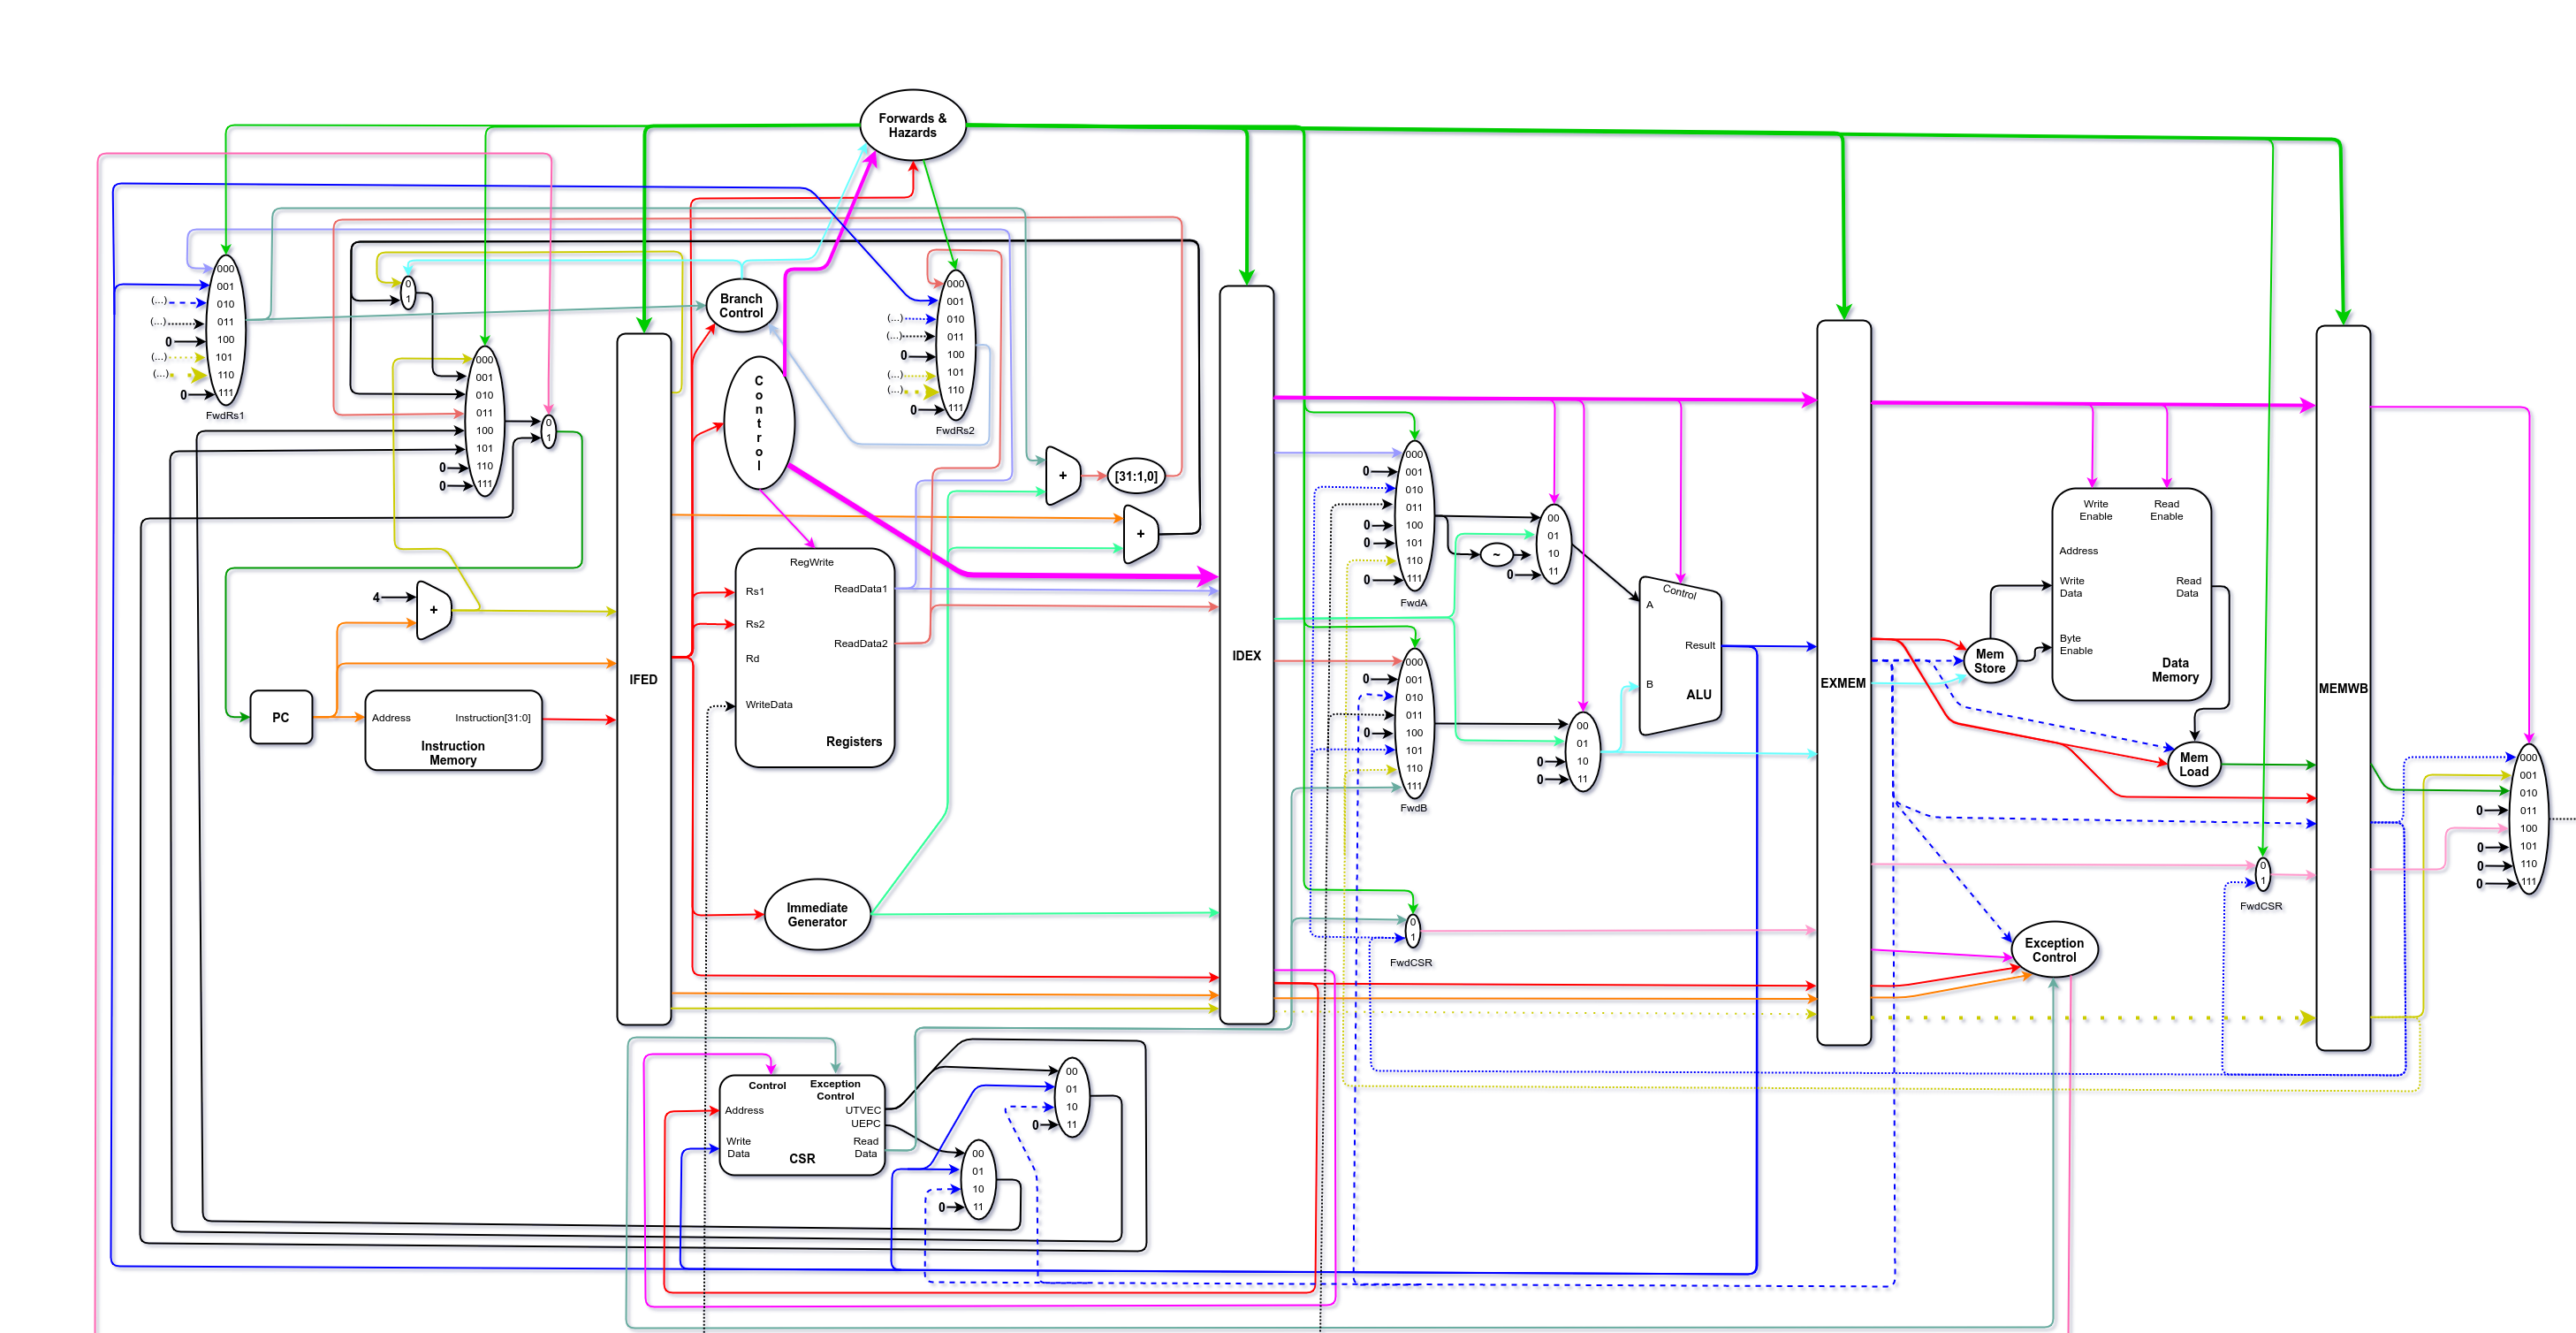
\includegraphics[angle=90,width=1\textwidth,height=1\textheight,keepaspectratio]{../images/uarch_diagrams/pipeline-RV32I-RV32IM.png}
    \caption{Diagrama do \textit{pipeline RV32I e RV32IM}}
\end{figure}

\begin{figure}[H]
\centering
    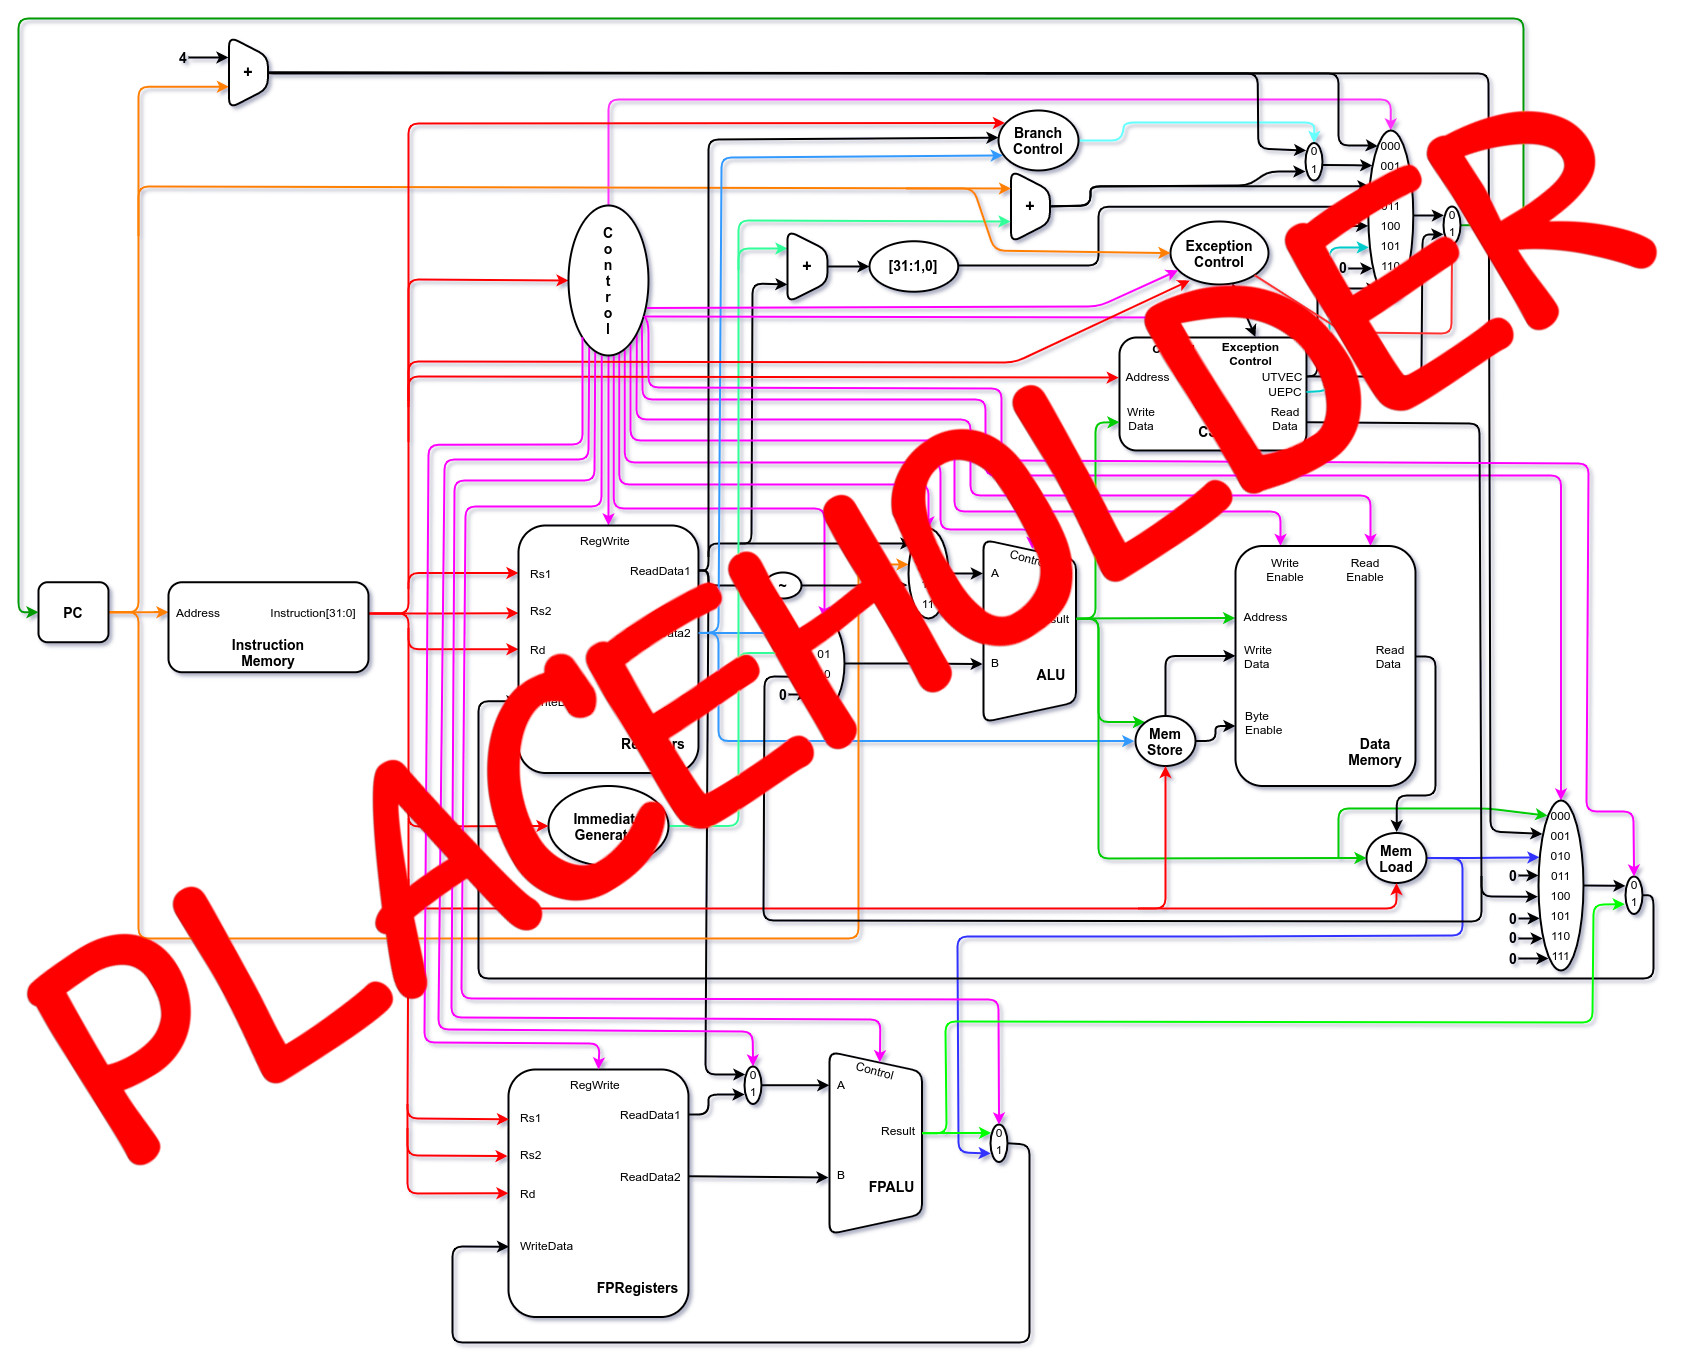
\includegraphics[angle=90,width=1\textwidth,height=1\textheight,keepaspectratio]{../images/uarch_diagrams/pipeline-RV32IMF.png}
    \caption{Diagrama do \textit{pipeline RV32IMF}}
\end{figure}

